\part{Raytracing}
\section{Optix}

\subsection{Introduction}
OptiX is a closed source raytracing engine designed by Nvidia, and currently only works on their own GPUs. The library is free to use both for hobbyists and for commerce. One can speculate that it will be opened up further once equivalent vendor agnostic libraries become available.

Optix can be seen as a framework for launching rays. It doesn't know anything about lights, shadows, ambient occlusion or any other rendering detail for that matter. What it does know is; rays, how to build and traverse acceleration structures, geometry representation and how to traverse the scene.What makes OptiX interesting is programmability; a variety of ray tracing-based algorithms in graphics and non-graphics domains can be implemented \cite{Parker10OptiX} by creating custom programs.

\subsection{Programs}
\paragraph{There are eight} different types of user provided programs in OptiX. These programs are implemented using the CUDA C-language. They all operate on a single ray at a time, except for the bounds program, which is used to determine bounds for acceleration structure construction. For triangle geometry, Optix can access individual vertices of a mesh for constructing a k-dimensional-tree (kdtree) or split bounding volume hierarchy  (sbvh).

\begin{enumerate}
	\item {
	\textbf{Ray generation}
      programs (``raygen'' from here on) are launched by the client program using rtContextLaunch(rayProgramIndex, with, height). This invokes many raygen programs in parallel. The raygen is the main entry point into the raytracing pipeline. Input and output buffers are declared inside. You can use a single raygen program as a general compute shader, but the intended use is to implement a camera model by initializing ray origin and direction. After a ray has been initialized, \begin{verbatim}rtTrace startNode,ray,payload \end{verbatim} can be called, and will trace all of start nodes children. 
	}

	\item{\textbf{Exeption} programs are invoked when the system encounters problems like out of stack space, or buffer access index is out of range. Also supports user-defined exceptions that can be 	thrown from any program. Can react by printing diagnostic messages or   writing specific color values to an output buffer.}

	\item{\textbf{Closest hit} programs are invoked once traversal has found the closest intersection of a ray with scene geometry. Surface shading is usually done in a closest hit program. Fragment color information is returned to the raygen program and stored in a buffer (for example a renderbuffer for further manipulation or a framebuffer).}

	\item{\textbf{Any hit}
		allow shading to be kept separate from geometry.
		May call rtTerminateRay and stop all traversal. Early ray termination for shadowrays and AO.
		Also useful for binary transparency by texture look up.
		Default any hit program is a no-op, often the most desired operation.
		}

	\item{\textbf{Miss} intersect any geometry. Typically used for enviroment map lookup or background color. }

	\item {\textbf{Intersection}
	programs are needed to describe geometry. The program must at least report if and where the ray touches the object, 
	additional computations may involve normals, texture coordinates and other attributes based on hit position.
	Intersection programs allow you to trace perfect spheres, cylinders, cubes,  CSG-surfaces, parametric surfaces like
	Bezier and NURBS, fractals and of course triangle meshes. Parker \cite{Parker10OptiX} notes \begin{quote} programmable intersection op-
	eration facilitates direct access to the native format, which can help
	avoid copies when interoperating with rasterization-based systems.\end{quote} In our program we store vertex attributes continuously (first all positions, then all normals, etc.) as opposed to storing them interleaved (one position, one normal and so on). Unfortunately, the built in acceleration sbvh and kdtree builders expect triangle geometry to be interleaved, so we settled for the generic bvh builder.
	}
	
	\item{\textbf{Selector}
		visit programs gives on control over graph traversal.
		The program can do traversals based on data stored in a visitor programs payload and make a traversal decision based 	on that data.
	}

 \item{\textbf{Bounding box}
		programs obviously compute the bounds associated with each primitive to enable acceleration structures over any geometry. The bounding box program takes a primtive index and computes its bounds. From the client api, a node is associated a given bounds program.
	}
 				
\end{enumerate}

The closest hit, any hit and miss programs determine shading. The raygen, selector and intersection programs determine scene traversal.
			 
\subsection{Client-side API}

To begin raytracing a scene ``rtContextLaunch( raygenIdx, width, height )'' is called with a given Rey Generation Program index as a parameter. From the ray generation program ``rtTrace( rootNode, ray, payload )'' is given the root scene node for traversal. During traversal, if a node a nodes associated selector and acceleration program is run.
If the acceleration traverser determines that a primitive node is hit, it invokes the primitives intersection program.
If the Intersection program calls ``rtReportIntersection'', the primitives associated ``material'' Any Hit Program is called.
If the ray doesn't hit anything, a miss program is called. The missprogram is always required.

	\begin{figure}[ht]
		\centering
		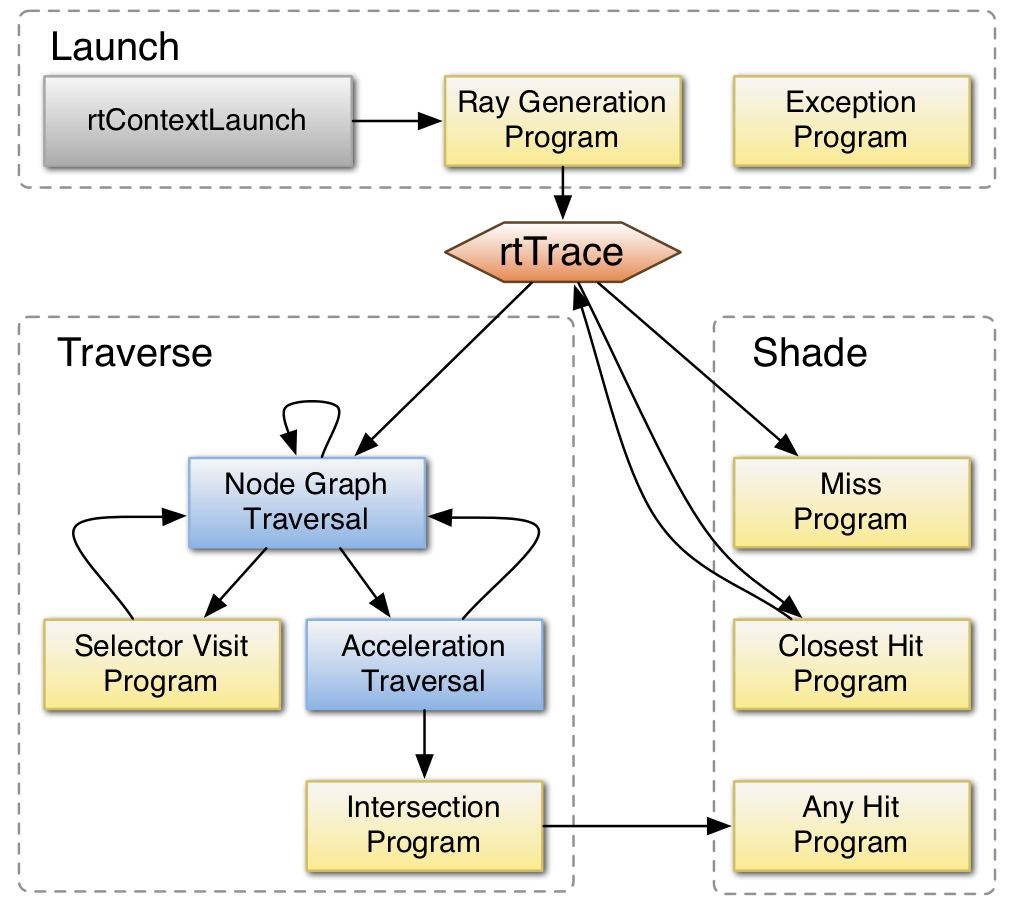
\includegraphics[width=0.50\textwidth]{Media/raytracer_optix_flow.png}
		\caption{Control flow through the ray tracing pipeline. Yellow boxes signify programmability. Blue boxes are algorithms internal to OptiX. Figure taken from \cite{Parker10OptiX} }
		\label{fig:pipelines}
	\end{figure}

\subsection{CUDA program API}

The simplest CUDA application only has one program; a raygen. The raygen program doesn't need to call rtTrace and can be used as a general CUDA program. See the code listing below \ref{raygen.cu} for a simple raygen program that implements a pinhole camera. The struct UserPayload payload is passed into the call to rtTrace, and is made available to the closest hit, any hit and miss programs when called during ray traversal.

\lstset{language=C++,caption={A simple raygen program},label=raygen.cu}
\begin{lstlisting}
// notice use of templates for type and dimension
rtBuffer<unsigned char, 2> outputBuffer; 

RT_PROGRAM void pinhole_camera() {
  Ray ray = PinholeCamera::makeRay( launchIndex );
  UserPayload payload;
  rtTrace( topObject, ray, payload );
  outputBuffer[launchIndex] = payload.result;
}
\end{lstlisting}